\documentclass[twoside]{book}

% Packages required by doxygen
\usepackage{fixltx2e}
\usepackage{calc}
\usepackage{doxygen}
\usepackage[export]{adjustbox} % also loads graphicx
\usepackage{graphicx}
\usepackage[utf8]{inputenc}
\usepackage{makeidx}
\usepackage{multicol}
\usepackage{multirow}
\PassOptionsToPackage{warn}{textcomp}
\usepackage{textcomp}
\usepackage[nointegrals]{wasysym}
\usepackage[table]{xcolor}

% Font selection
\usepackage[T1]{fontenc}
\usepackage[scaled=.90]{helvet}
\usepackage{courier}
\usepackage{amssymb}
\usepackage{sectsty}
\renewcommand{\familydefault}{\sfdefault}
\allsectionsfont{%
  \fontseries{bc}\selectfont%
  \color{darkgray}%
}
\renewcommand{\DoxyLabelFont}{%
  \fontseries{bc}\selectfont%
  \color{darkgray}%
}
\newcommand{\+}{\discretionary{\mbox{\scriptsize$\hookleftarrow$}}{}{}}

% Page & text layout
\usepackage{geometry}
\geometry{%
  a4paper,%
  top=2.5cm,%
  bottom=2.5cm,%
  left=2.5cm,%
  right=2.5cm%
}
\tolerance=750
\hfuzz=15pt
\hbadness=750
\setlength{\emergencystretch}{15pt}
\setlength{\parindent}{0cm}
\setlength{\parskip}{3ex plus 2ex minus 2ex}
\makeatletter
\renewcommand{\paragraph}{%
  \@startsection{paragraph}{4}{0ex}{-1.0ex}{1.0ex}{%
    \normalfont\normalsize\bfseries\SS@parafont%
  }%
}
\renewcommand{\subparagraph}{%
  \@startsection{subparagraph}{5}{0ex}{-1.0ex}{1.0ex}{%
    \normalfont\normalsize\bfseries\SS@subparafont%
  }%
}
\makeatother

% Headers & footers
\usepackage{fancyhdr}
\pagestyle{fancyplain}
\fancyhead[LE]{\fancyplain{}{\bfseries\thepage}}
\fancyhead[CE]{\fancyplain{}{}}
\fancyhead[RE]{\fancyplain{}{\bfseries\leftmark}}
\fancyhead[LO]{\fancyplain{}{\bfseries\rightmark}}
\fancyhead[CO]{\fancyplain{}{}}
\fancyhead[RO]{\fancyplain{}{\bfseries\thepage}}
\fancyfoot[LE]{\fancyplain{}{}}
\fancyfoot[CE]{\fancyplain{}{}}
\fancyfoot[RE]{\fancyplain{}{\bfseries\scriptsize Generated by Doxygen }}
\fancyfoot[LO]{\fancyplain{}{\bfseries\scriptsize Generated by Doxygen }}
\fancyfoot[CO]{\fancyplain{}{}}
\fancyfoot[RO]{\fancyplain{}{}}
\renewcommand{\footrulewidth}{0.4pt}
\renewcommand{\chaptermark}[1]{%
  \markboth{#1}{}%
}
\renewcommand{\sectionmark}[1]{%
  \markright{\thesection\ #1}%
}

% Indices & bibliography
\usepackage{natbib}
\usepackage[titles]{tocloft}
\setcounter{tocdepth}{3}
\setcounter{secnumdepth}{5}
\makeindex

% Hyperlinks (required, but should be loaded last)
\usepackage{ifpdf}
\ifpdf
  \usepackage[pdftex,pagebackref=true]{hyperref}
\else
  \usepackage[ps2pdf,pagebackref=true]{hyperref}
\fi
\hypersetup{%
  colorlinks=true,%
  linkcolor=blue,%
  citecolor=blue,%
  unicode%
}

% Custom commands
\newcommand{\clearemptydoublepage}{%
  \newpage{\pagestyle{empty}\cleardoublepage}%
}

\usepackage{caption}
\captionsetup{labelsep=space,justification=centering,font={bf},singlelinecheck=off,skip=4pt,position=top}

%===== C O N T E N T S =====

\begin{document}

% Titlepage & ToC
\hypersetup{pageanchor=false,
             bookmarksnumbered=true,
             pdfencoding=unicode
            }
\pagenumbering{roman}
\begin{titlepage}
\vspace*{7cm}
\begin{center}%
{\Large Orange Ball \\[1ex]\large 0.\+0.\+1 }\\
\vspace*{1cm}
{\large Generated by Doxygen 1.8.11}\\
\end{center}
\end{titlepage}
\clearemptydoublepage
\tableofcontents
\clearemptydoublepage
\pagenumbering{arabic}
\hypersetup{pageanchor=true}

%--- Begin generated contents ---
\chapter{Kameraerkennung für den Orangenen Ball}
\label{md_README}
\hypertarget{md_README}{}
\subsection*{In}
\chapter{Class Index}
\section{Class List}
Here are the classes, structs, unions and interfaces with brief descriptions\+:\begin{DoxyCompactList}
\item\contentsline{section}{\hyperlink{classCircleFinderResult}{Circle\+Finder\+Result} }{\pageref{d1/da1/classCircleFinderResult}}{}
\item\contentsline{section}{\hyperlink{classLine}{Line} }{\pageref{db/db6/classLine}}{}
\end{DoxyCompactList}

\chapter{File Index}
\section{File List}
Here is a list of all documented files with brief descriptions\+:\begin{DoxyCompactList}
\item\contentsline{section}{\hyperlink{Canny_8hpp}{Canny.\+hpp} }{\pageref{d1/d5a/Canny_8hpp}}{}
\item\contentsline{section}{\hyperlink{CircleFinder_8hpp}{Circle\+Finder.\+hpp} }{\pageref{d7/daa/CircleFinder_8hpp}}{}
\item\contentsline{section}{{\bfseries Circle\+Finder\+Result.\+hpp} }{\pageref{dd/d2f/CircleFinderResult_8hpp}}{}
\item\contentsline{section}{\hyperlink{ColourBased_8hpp}{Colour\+Based.\+hpp} }{\pageref{d4/de5/ColourBased_8hpp}}{}
\item\contentsline{section}{\hyperlink{Line_8cpp}{Line.\+cpp} }{\pageref{d4/dae/Line_8cpp}}{}
\item\contentsline{section}{\hyperlink{Line_8hpp}{Line.\+hpp} }{\pageref{db/d57/Line_8hpp}}{}
\item\contentsline{section}{\hyperlink{main_8cpp}{main.\+cpp} \\*Main file }{\pageref{df/d0a/main_8cpp}}{}
\end{DoxyCompactList}

\chapter{Class Documentation}
\hypertarget{classCircleFinderResult}{}\section{Circle\+Finder\+Result Class Reference}
\label{classCircleFinderResult}\index{Circle\+Finder\+Result@{Circle\+Finder\+Result}}
\subsection*{Public Member Functions}
\begin{DoxyCompactItemize}
\item 
{\bfseries Circle\+Finder\+Result} (bool is\+Circle)\hypertarget{classCircleFinderResult_ad07edae86537838f212e586595e05b00}{}\label{classCircleFinderResult_ad07edae86537838f212e586595e05b00}

\item 
{\bfseries Circle\+Finder\+Result} (Point centre, int radius, bool is\+Circle)\hypertarget{classCircleFinderResult_a520a0d45adf3ed5700f87f3eabdbe97c}{}\label{classCircleFinderResult_a520a0d45adf3ed5700f87f3eabdbe97c}

\end{DoxyCompactItemize}
\subsection*{Public Attributes}
\begin{DoxyCompactItemize}
\item 
Point {\bfseries centre}\hypertarget{classCircleFinderResult_a5e521162d00f1c37484017274595037e}{}\label{classCircleFinderResult_a5e521162d00f1c37484017274595037e}

\item 
int {\bfseries radius}\hypertarget{classCircleFinderResult_a8b184dfa60cfff1403ef9eef5258abdc}{}\label{classCircleFinderResult_a8b184dfa60cfff1403ef9eef5258abdc}

\item 
bool {\bfseries is\+Circle}\hypertarget{classCircleFinderResult_a1c6eeba1874d040f770791f8779f666a}{}\label{classCircleFinderResult_a1c6eeba1874d040f770791f8779f666a}

\end{DoxyCompactItemize}


The documentation for this class was generated from the following files\+:\begin{DoxyCompactItemize}
\item 
Circle\+Finder\+Result.\+hpp\item 
Circle\+Finder\+Result.\+cpp\end{DoxyCompactItemize}

\hypertarget{classLine}{}\section{Line Class Reference}
\label{classLine}\index{Line@{Line}}
\subsection*{Public Member Functions}
\begin{DoxyCompactItemize}
\item 
\hyperlink{classLine_afeaa676c7d249d582c5766dc732a78e2}{Line} (Point p1, Point p2)
\item 
\hyperlink{classLine_ae803f230922e370616841c934948d6de}{Line} (Point p, double m)
\item 
\hyperlink{classLine}{Line} \hyperlink{classLine_a4cfed9ec6c5f078db5fe45b7df201c0c}{get\+Inverted} (Point p)
\item 
double \hyperlink{classLine_a872b756c94ed478d05e430ebb436b116}{get\+Gradient} ()
\item 
bool \hyperlink{classLine_aabb022cbf0d8b18e011058c43d1b8290}{exists\+Intersection} (\hyperlink{classLine}{Line} line)
\item 
Point \hyperlink{classLine_abe8bb540dbdd9376eed3ba29f9beee51}{get\+Intersection} (\hyperlink{classLine}{Line} line)
\item 
int \hyperlink{classLine_abc0b1133b03c85072b1ca7d3f650915b}{getY} (int x)
\item 
int \hyperlink{classLine_a16167c02532f44bcba31a5c158629a56}{getC} ()
\item 
int \hyperlink{classLine_ae82bab13355161079a09e2fcd1b4fc1c}{get\+Dist\+Points} ()
\end{DoxyCompactItemize}


\subsection{Constructor \& Destructor Documentation}
\index{Line@{Line}!Line@{Line}}
\index{Line@{Line}!Line@{Line}}
\subsubsection[{\texorpdfstring{Line(\+Point p1, Point p2)}{Line(Point p1, Point p2)}}]{\setlength{\rightskip}{0pt plus 5cm}Line\+::\+Line (
\begin{DoxyParamCaption}
\item[{Point}]{p1, }
\item[{Point}]{p2}
\end{DoxyParamCaption}
)}\hypertarget{classLine_afeaa676c7d249d582c5766dc732a78e2}{}\label{classLine_afeaa676c7d249d582c5766dc732a78e2}
Constructor\+: define a \hyperlink{classLine}{Line} through two points 
\begin{DoxyParams}{Parameters}
{\em p1} & the first point the line should go through \\
\hline
{\em p2} & the second point the line should go through \\
\hline
\end{DoxyParams}
\index{Line@{Line}!Line@{Line}}
\index{Line@{Line}!Line@{Line}}
\subsubsection[{\texorpdfstring{Line(\+Point p, double m)}{Line(Point p, double m)}}]{\setlength{\rightskip}{0pt plus 5cm}Line\+::\+Line (
\begin{DoxyParamCaption}
\item[{Point}]{p, }
\item[{double}]{m}
\end{DoxyParamCaption}
)}\hypertarget{classLine_ae803f230922e370616841c934948d6de}{}\label{classLine_ae803f230922e370616841c934948d6de}
Constructor\+: define a \hyperlink{classLine}{Line} through a point and a gradient 
\begin{DoxyParams}{Parameters}
{\em p} & the point the line should go through \\
\hline
{\em m} & the gradient of the line \\
\hline
\end{DoxyParams}


\subsection{Member Function Documentation}
\index{Line@{Line}!exists\+Intersection@{exists\+Intersection}}
\index{exists\+Intersection@{exists\+Intersection}!Line@{Line}}
\subsubsection[{\texorpdfstring{exists\+Intersection(\+Line line)}{existsIntersection(Line line)}}]{\setlength{\rightskip}{0pt plus 5cm}bool Line\+::exists\+Intersection (
\begin{DoxyParamCaption}
\item[{{\bf Line}}]{line}
\end{DoxyParamCaption}
)}\hypertarget{classLine_aabb022cbf0d8b18e011058c43d1b8290}{}\label{classLine_aabb022cbf0d8b18e011058c43d1b8290}
Check if an intersection between two lines exists 
\begin{DoxyParams}{Parameters}
{\em line} & the second line \\
\hline
\end{DoxyParams}
\begin{DoxyReturn}{Returns}
a boolean which is true if there is a well-\/defined intersection 
\end{DoxyReturn}
\index{Line@{Line}!getC@{getC}}
\index{getC@{getC}!Line@{Line}}
\subsubsection[{\texorpdfstring{get\+C()}{getC()}}]{\setlength{\rightskip}{0pt plus 5cm}int Line\+::getC (
\begin{DoxyParamCaption}
{}
\end{DoxyParamCaption}
)}\hypertarget{classLine_a16167c02532f44bcba31a5c158629a56}{}\label{classLine_a16167c02532f44bcba31a5c158629a56}
Get the Y value at x=0 \begin{DoxyReturn}{Returns}
the y value of the line at x=0 
\end{DoxyReturn}
\index{Line@{Line}!get\+Dist\+Points@{get\+Dist\+Points}}
\index{get\+Dist\+Points@{get\+Dist\+Points}!Line@{Line}}
\subsubsection[{\texorpdfstring{get\+Dist\+Points()}{getDistPoints()}}]{\setlength{\rightskip}{0pt plus 5cm}int Line\+::get\+Dist\+Points (
\begin{DoxyParamCaption}
{}
\end{DoxyParamCaption}
)}\hypertarget{classLine_ae82bab13355161079a09e2fcd1b4fc1c}{}\label{classLine_ae82bab13355161079a09e2fcd1b4fc1c}
Get the distance of the two points which define the line (similar to a normal abs function of a line with limited length) \begin{DoxyReturn}{Returns}
the distance of both points which were used to define the line 
\end{DoxyReturn}
\index{Line@{Line}!get\+Gradient@{get\+Gradient}}
\index{get\+Gradient@{get\+Gradient}!Line@{Line}}
\subsubsection[{\texorpdfstring{get\+Gradient()}{getGradient()}}]{\setlength{\rightskip}{0pt plus 5cm}double Line\+::get\+Gradient (
\begin{DoxyParamCaption}
{}
\end{DoxyParamCaption}
)}\hypertarget{classLine_a872b756c94ed478d05e430ebb436b116}{}\label{classLine_a872b756c94ed478d05e430ebb436b116}
Get the current gradient of the line (dx/dy) \begin{DoxyReturn}{Returns}
the gradient of the line, return N\+AN if the line is vertical (-\/$>$ gradient is infinity) 
\end{DoxyReturn}
\index{Line@{Line}!get\+Intersection@{get\+Intersection}}
\index{get\+Intersection@{get\+Intersection}!Line@{Line}}
\subsubsection[{\texorpdfstring{get\+Intersection(\+Line line)}{getIntersection(Line line)}}]{\setlength{\rightskip}{0pt plus 5cm}Point Line\+::get\+Intersection (
\begin{DoxyParamCaption}
\item[{{\bf Line}}]{line}
\end{DoxyParamCaption}
)}\hypertarget{classLine_abe8bb540dbdd9376eed3ba29f9beee51}{}\label{classLine_abe8bb540dbdd9376eed3ba29f9beee51}
Get the intersection of the current line with the given line, always check exists\+Intersection before! 
\begin{DoxyParams}{Parameters}
{\em line} & the current line should check the intersection with \\
\hline
\end{DoxyParams}
\begin{DoxyReturn}{Returns}
the point both lines are intersecting 
\end{DoxyReturn}
\index{Line@{Line}!get\+Inverted@{get\+Inverted}}
\index{get\+Inverted@{get\+Inverted}!Line@{Line}}
\subsubsection[{\texorpdfstring{get\+Inverted(\+Point p)}{getInverted(Point p)}}]{\setlength{\rightskip}{0pt plus 5cm}{\bf Line} Line\+::get\+Inverted (
\begin{DoxyParamCaption}
\item[{Point}]{p}
\end{DoxyParamCaption}
)}\hypertarget{classLine_a4cfed9ec6c5f078db5fe45b7df201c0c}{}\label{classLine_a4cfed9ec6c5f078db5fe45b7df201c0c}
Get the line in 90deg angle to the \hyperlink{classLine}{Line} 
\begin{DoxyParams}{Parameters}
{\em p} & the point the line should go through \\
\hline
\end{DoxyParams}
\begin{DoxyReturn}{Returns}
a new \hyperlink{classLine}{Line} which intersects the \hyperlink{classLine}{Line} in the given point 
\end{DoxyReturn}
\index{Line@{Line}!getY@{getY}}
\index{getY@{getY}!Line@{Line}}
\subsubsection[{\texorpdfstring{get\+Y(int x)}{getY(int x)}}]{\setlength{\rightskip}{0pt plus 5cm}int Line\+::getY (
\begin{DoxyParamCaption}
\item[{int}]{x}
\end{DoxyParamCaption}
)}\hypertarget{classLine_abc0b1133b03c85072b1ca7d3f650915b}{}\label{classLine_abc0b1133b03c85072b1ca7d3f650915b}
Get the y value of the line at a certain x position 
\begin{DoxyParams}{Parameters}
{\em x} & the x value the y value should be calculated \\
\hline
\end{DoxyParams}
\begin{DoxyReturn}{Returns}
the y value of the line, or -\/1 if the line is vertical 
\end{DoxyReturn}


The documentation for this class was generated from the following files\+:\begin{DoxyCompactItemize}
\item 
Line.\+hpp\item 
Line.\+cpp\end{DoxyCompactItemize}

\chapter{File Documentation}
\hypertarget{Canny_8hpp}{}\section{Canny.\+hpp File Reference}
\label{Canny_8hpp}\index{Canny.\+hpp@{Canny.\+hpp}}
{\ttfamily \#include \char`\"{}Circle\+Finder.\+hpp\char`\"{}}\\*
Include dependency graph for Canny.\+hpp\+:
\nopagebreak
\begin{figure}[H]
\begin{center}
\leavevmode
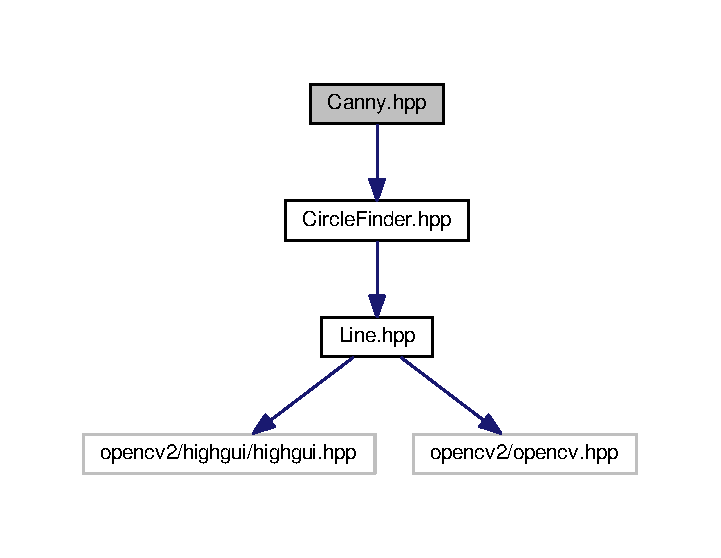
\includegraphics[width=346pt]{df/daa/Canny_8hpp__incl}
\end{center}
\end{figure}
This graph shows which files directly or indirectly include this file\+:\nopagebreak
\begin{figure}[H]
\begin{center}
\leavevmode
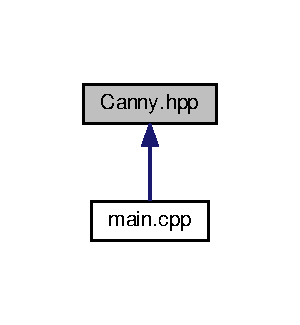
\includegraphics[width=144pt]{dc/dfe/Canny_8hpp__dep__incl}
\end{center}
\end{figure}
\subsection*{Functions}
\begin{DoxyCompactItemize}
\item 
void {\bfseries cnny\+::init} ()\hypertarget{Canny_8hpp_aca5a1444c0b06cb8e090a40030fc01c3}{}\label{Canny_8hpp_aca5a1444c0b06cb8e090a40030fc01c3}

\item 
void {\bfseries cnny\+::close} ()\hypertarget{Canny_8hpp_a2bd2c98aa9f98b1a8b7b4646a7794915}{}\label{Canny_8hpp_a2bd2c98aa9f98b1a8b7b4646a7794915}

\item 
void {\bfseries cnny\+::show} (Mat img)\hypertarget{Canny_8hpp_a8489b6c074e3fa3a3f112eb55d8d158b}{}\label{Canny_8hpp_a8489b6c074e3fa3a3f112eb55d8d158b}

\item 
Mat {\bfseries cnny\+::run} (Mat img\+Original)\hypertarget{Canny_8hpp_aabcca0335e06ee1d8c939d40d0e1adea}{}\label{Canny_8hpp_aabcca0335e06ee1d8c939d40d0e1adea}

\end{DoxyCompactItemize}
\subsection*{Variables}
\begin{DoxyCompactItemize}
\item 
int {\bfseries cnny\+::threshold}\hypertarget{Canny_8hpp_a7ba9841638cbf21a6bb15ee81b36871c}{}\label{Canny_8hpp_a7ba9841638cbf21a6bb15ee81b36871c}

\end{DoxyCompactItemize}


\subsection{Detailed Description}
\begin{DoxyAuthor}{Author}
Paul Nykiel, Tim Luchterhand 
\end{DoxyAuthor}

\hypertarget{CircleFinder_8hpp}{}\section{Circle\+Finder.\+hpp File Reference}
\label{CircleFinder_8hpp}\index{Circle\+Finder.\+hpp@{Circle\+Finder.\+hpp}}
{\ttfamily \#include \char`\"{}Line.\+hpp\char`\"{}}\\*
Include dependency graph for Circle\+Finder.\+hpp\+:
\nopagebreak
\begin{figure}[H]
\begin{center}
\leavevmode
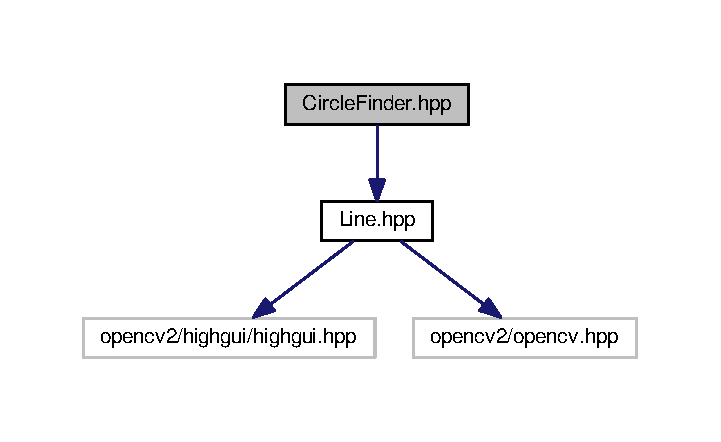
\includegraphics[width=346pt]{d5/d55/CircleFinder_8hpp__incl}
\end{center}
\end{figure}
This graph shows which files directly or indirectly include this file\+:\nopagebreak
\begin{figure}[H]
\begin{center}
\leavevmode
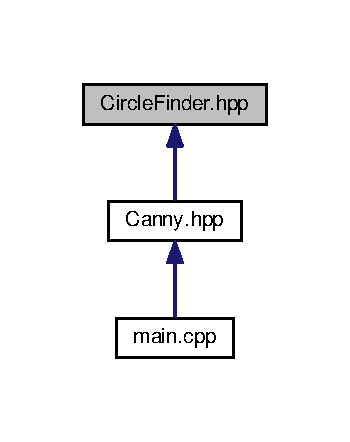
\includegraphics[width=168pt]{d7/d9a/CircleFinder_8hpp__dep__incl}
\end{center}
\end{figure}
\subsection*{Macros}
\begin{DoxyCompactItemize}
\item 
\#define {\bfseries SQ}(x)~(x$\ast$x)\hypertarget{CircleFinder_8hpp_ac3644f84794a8bfdacf39c4b2c2495fc}{}\label{CircleFinder_8hpp_ac3644f84794a8bfdacf39c4b2c2495fc}

\end{DoxyCompactItemize}
\subsection*{Functions}
\begin{DoxyCompactItemize}
\item 
int {\bfseries crclfnd\+::sq\+Distance} (Point p1, Point p2)\hypertarget{CircleFinder_8hpp_ac6e5df61443e2d1f28a30f73e536f525}{}\label{CircleFinder_8hpp_ac6e5df61443e2d1f28a30f73e536f525}

\item 
Point {\bfseries crclfnd\+::get\+Middle} (Point p1, Point p2)\hypertarget{CircleFinder_8hpp_a0cf534d99d610da43f11b2c79d5756fd}{}\label{CircleFinder_8hpp_a0cf534d99d610da43f11b2c79d5756fd}

\item 
Point {\bfseries crclfnd\+::get\+Middle} (Point p1, Point p2, Point p3)\hypertarget{CircleFinder_8hpp_abdc6cf60dffa7f0b8ce3366915702b95}{}\label{CircleFinder_8hpp_abdc6cf60dffa7f0b8ce3366915702b95}

\item 
int {\bfseries crclfnd\+::get\+Point\+Distance} (Point check, Point p1, Point p2)\hypertarget{CircleFinder_8hpp_a6d4553da7823ef1912a741dd13660d94}{}\label{CircleFinder_8hpp_a6d4553da7823ef1912a741dd13660d94}

\item 
bool {\bfseries crclfnd\+::is\+Circle} (std\+::vector$<$ Point $>$ points)\hypertarget{CircleFinder_8hpp_abfa368c61933116fe21786fd1b727b97}{}\label{CircleFinder_8hpp_abfa368c61933116fe21786fd1b727b97}

\end{DoxyCompactItemize}
\subsection*{Variables}
\begin{DoxyCompactItemize}
\item 
int \hyperlink{CircleFinder_8hpp_aed6d70cdca12c6712825ba4e60d0011a}{crclfnd\+::minimum\+Points} = 10\hypertarget{CircleFinder_8hpp_aed6d70cdca12c6712825ba4e60d0011a}{}\label{CircleFinder_8hpp_aed6d70cdca12c6712825ba4e60d0011a}

\begin{DoxyCompactList}\small\item\em Minimum Points required for a form to be allowed as a circle. \end{DoxyCompactList}\item 
double {\bfseries crclfnd\+::cos45} = 0.\+707106781186547524400\hypertarget{CircleFinder_8hpp_ad891cf76862264a3e7e1d0f3e07d7560}{}\label{CircleFinder_8hpp_ad891cf76862264a3e7e1d0f3e07d7560}

\item 
int {\bfseries crclfnd\+::max\+Radius} = 500\hypertarget{CircleFinder_8hpp_abc8bbaa6c3a09647e46059bc2c8ea45e}{}\label{CircleFinder_8hpp_abc8bbaa6c3a09647e46059bc2c8ea45e}

\item 
int {\bfseries crclfnd\+::distance\+Threshold} = SQ(50)\hypertarget{CircleFinder_8hpp_adb7105456bd81200afff0d0a3579dfc6}{}\label{CircleFinder_8hpp_adb7105456bd81200afff0d0a3579dfc6}

\item 
int {\bfseries crclfnd\+::circle\+Center\+Distance\+Threshold} = SQ(25)\hypertarget{CircleFinder_8hpp_ae9cf805faa485d5bad0fa521fd47d18d}{}\label{CircleFinder_8hpp_ae9cf805faa485d5bad0fa521fd47d18d}

\item 
double {\bfseries crclfnd\+::radius\+Ratio\+Threshold} = 0.\+1\hypertarget{CircleFinder_8hpp_ac317772b445831ea31329f14709e6ca6}{}\label{CircleFinder_8hpp_ac317772b445831ea31329f14709e6ca6}

\end{DoxyCompactItemize}


\subsection{Detailed Description}
\begin{DoxyAuthor}{Authors}
Paul Nykiel, Tim Luchterhand 
\end{DoxyAuthor}

\hypertarget{ColourBased_8hpp}{}\section{Colour\+Based.\+hpp File Reference}
\label{ColourBased_8hpp}\index{Colour\+Based.\+hpp@{Colour\+Based.\+hpp}}
This graph shows which files directly or indirectly include this file\+:
\nopagebreak
\begin{figure}[H]
\begin{center}
\leavevmode
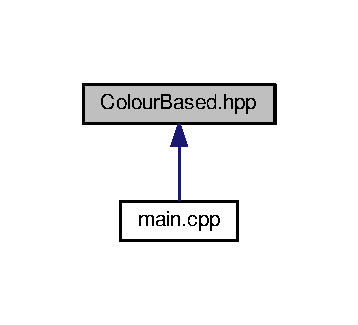
\includegraphics[width=172pt]{d6/d69/ColourBased_8hpp__dep__incl}
\end{center}
\end{figure}
\subsection*{Functions}
\begin{DoxyCompactItemize}
\item 
void {\bfseries clr\+::init} ()\hypertarget{ColourBased_8hpp_aed37bb6d4af11bfaf42b81f06e3c099e}{}\label{ColourBased_8hpp_aed37bb6d4af11bfaf42b81f06e3c099e}

\item 
void {\bfseries clr\+::close} ()\hypertarget{ColourBased_8hpp_ac6598b50de4dd5854a2ac5e5df51687a}{}\label{ColourBased_8hpp_ac6598b50de4dd5854a2ac5e5df51687a}

\item 
void {\bfseries clr\+::show} (Mat img)\hypertarget{ColourBased_8hpp_ad73bdacd64c62f31f06c8b1a2c7e09d3}{}\label{ColourBased_8hpp_ad73bdacd64c62f31f06c8b1a2c7e09d3}

\item 
bool {\bfseries clr\+::compare\+Contour\+Areas} (std\+::vector$<$ cv\+::\+Point $>$ contour1, std\+::vector$<$ cv\+::\+Point $>$ contour2)\hypertarget{ColourBased_8hpp_a490facc8b0b18415d7e1d316dbebee06}{}\label{ColourBased_8hpp_a490facc8b0b18415d7e1d316dbebee06}

\item 
Mat {\bfseries clr\+::run} (Mat img\+Original)\hypertarget{ColourBased_8hpp_accc2d4f4291ae1f36184b5cef4e81f69}{}\label{ColourBased_8hpp_accc2d4f4291ae1f36184b5cef4e81f69}

\end{DoxyCompactItemize}
\subsection*{Variables}
\begin{DoxyCompactItemize}
\item 
int {\bfseries clr\+::min\+Hue}\hypertarget{ColourBased_8hpp_a7978af6eb69d3d2f5971ba40c06b2aed}{}\label{ColourBased_8hpp_a7978af6eb69d3d2f5971ba40c06b2aed}

\item 
int {\bfseries clr\+::max\+Hue}\hypertarget{ColourBased_8hpp_a8ea47f3b918e912efa1492d3b39cffd1}{}\label{ColourBased_8hpp_a8ea47f3b918e912efa1492d3b39cffd1}

\item 
int {\bfseries clr\+::min\+Saturation}\hypertarget{ColourBased_8hpp_abde1e9c05bc8a6b41501965699a4b1a0}{}\label{ColourBased_8hpp_abde1e9c05bc8a6b41501965699a4b1a0}

\item 
int {\bfseries clr\+::max\+Saturation}\hypertarget{ColourBased_8hpp_a3c2d6bd84c3ad2e0fee5c11c9f583650}{}\label{ColourBased_8hpp_a3c2d6bd84c3ad2e0fee5c11c9f583650}

\item 
int {\bfseries clr\+::min\+Value}\hypertarget{ColourBased_8hpp_a24f1d95cd6b26523dbd3c4423aae7260}{}\label{ColourBased_8hpp_a24f1d95cd6b26523dbd3c4423aae7260}

\item 
int {\bfseries clr\+::max\+Value}\hypertarget{ColourBased_8hpp_a6481be70f57e7359f622eb1ab29f5299}{}\label{ColourBased_8hpp_a6481be70f57e7359f622eb1ab29f5299}

\item 
int {\bfseries clr\+::min\+Size}\hypertarget{ColourBased_8hpp_aa1aaab5c27fe7367d2f742306e6a56fd}{}\label{ColourBased_8hpp_aa1aaab5c27fe7367d2f742306e6a56fd}

\end{DoxyCompactItemize}


\subsection{Detailed Description}
\begin{DoxyAuthor}{Author}
Paul Nykiel, Tim Luchterhand 
\end{DoxyAuthor}

\hypertarget{Line_8cpp}{}\section{Line.\+cpp File Reference}
\label{Line_8cpp}\index{Line.\+cpp@{Line.\+cpp}}
{\ttfamily \#include $<$cmath$>$}\\*
{\ttfamily \#include \char`\"{}Line.\+hpp\char`\"{}}\\*
Include dependency graph for Line.\+cpp\+:
\nopagebreak
\begin{figure}[H]
\begin{center}
\leavevmode
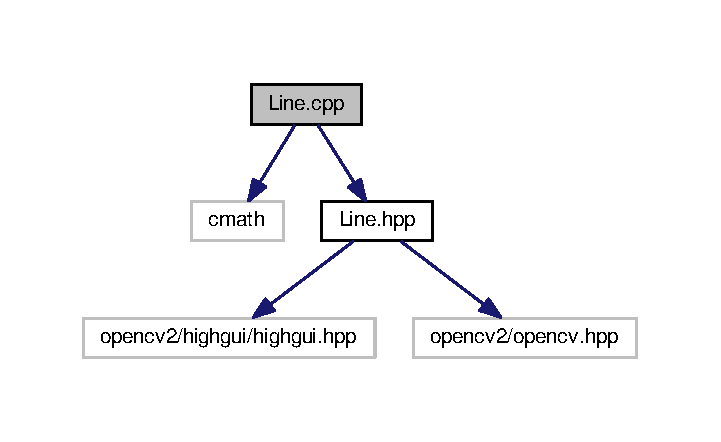
\includegraphics[width=346pt]{d2/d2b/Line_8cpp__incl}
\end{center}
\end{figure}


\subsection{Detailed Description}
\begin{DoxyAuthor}{Author}
Paul Nykiel, Tim Luchterhand 
\end{DoxyAuthor}

\hypertarget{Line_8hpp}{}\section{Line.\+hpp File Reference}
\label{Line_8hpp}\index{Line.\+hpp@{Line.\+hpp}}
{\ttfamily \#include \char`\"{}opencv2/highgui/highgui.\+hpp\char`\"{}}\\*
{\ttfamily \#include \char`\"{}opencv2/opencv.\+hpp\char`\"{}}\\*
Include dependency graph for Line.\+hpp\+:
\nopagebreak
\begin{figure}[H]
\begin{center}
\leavevmode
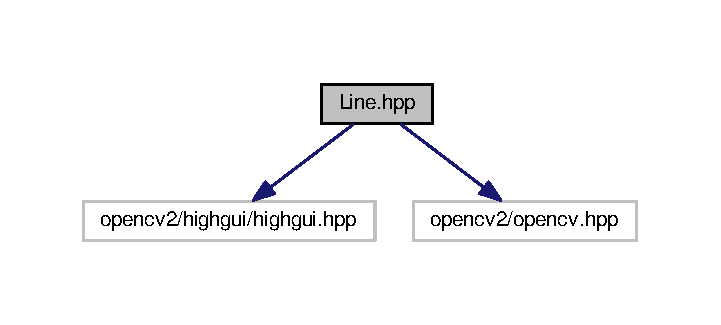
\includegraphics[width=346pt]{db/dd2/Line_8hpp__incl}
\end{center}
\end{figure}
This graph shows which files directly or indirectly include this file\+:
\nopagebreak
\begin{figure}[H]
\begin{center}
\leavevmode
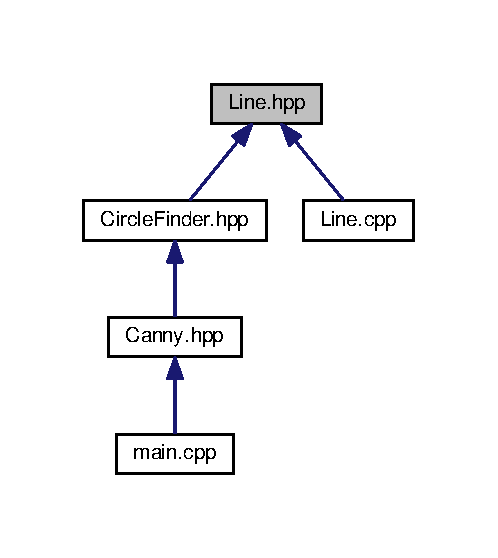
\includegraphics[width=239pt]{d4/d39/Line_8hpp__dep__incl}
\end{center}
\end{figure}
\subsection*{Classes}
\begin{DoxyCompactItemize}
\item 
class \hyperlink{classLine}{Line}
\end{DoxyCompactItemize}


\subsection{Detailed Description}
\begin{DoxyAuthor}{Author}
Paul Nykiel, Tim Luchterhand 
\end{DoxyAuthor}

\hypertarget{main_8cpp}{}\section{main.\+cpp File Reference}
\label{main_8cpp}\index{main.\+cpp@{main.\+cpp}}


Main file.  


{\ttfamily \#include $<$iostream$>$}\\*
{\ttfamily \#include $<$thread$>$}\\*
{\ttfamily \#include \char`\"{}opencv2/highgui/highgui.\+hpp\char`\"{}}\\*
{\ttfamily \#include \char`\"{}opencv2/opencv.\+hpp\char`\"{}}\\*
{\ttfamily \#include \char`\"{}Colour\+Based.\+hpp\char`\"{}}\\*
{\ttfamily \#include \char`\"{}Canny.\+hpp\char`\"{}}\\*
{\ttfamily \#include \char`\"{}Hough\+Circle.\+hpp\char`\"{}}\\*
Include dependency graph for main.\+cpp\+:
\nopagebreak
\begin{figure}[H]
\begin{center}
\leavevmode
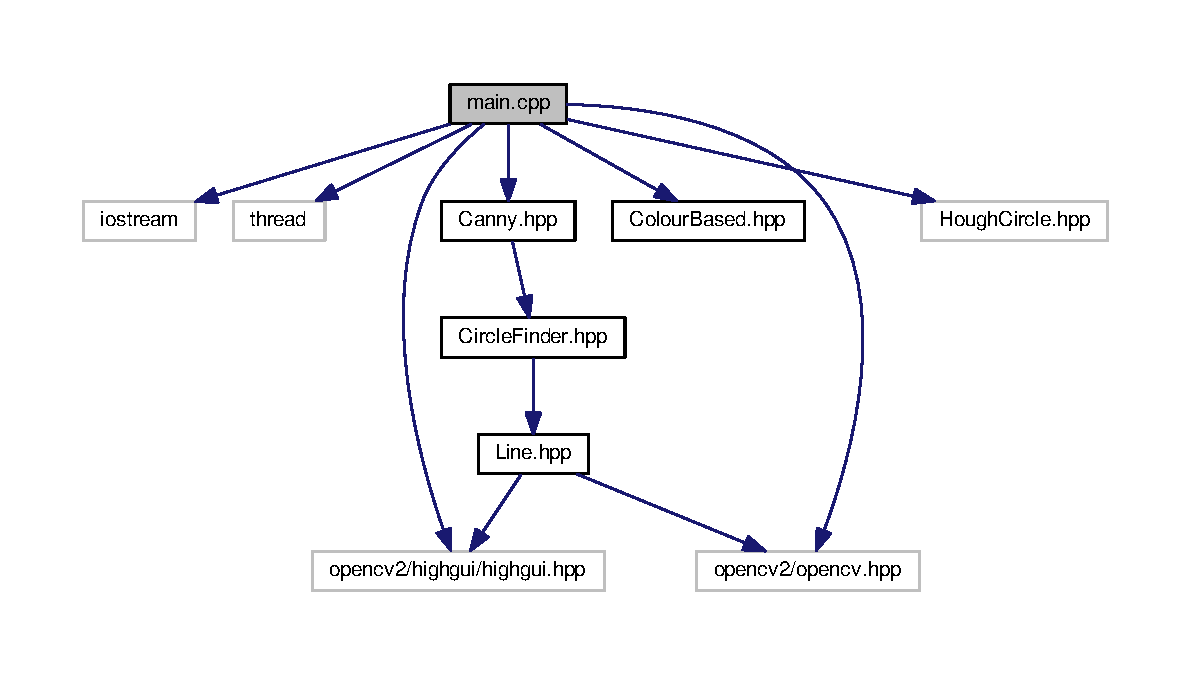
\includegraphics[width=350pt]{da/dce/main_8cpp__incl}
\end{center}
\end{figure}
\subsection*{Functions}
\begin{DoxyCompactItemize}
\item 
void \hyperlink{main_8cpp_aaad3480f7b14479833136e922e72bb33}{on\+Mouse\+Original\+Click} (int event, int x, int y, int, void $\ast$)
\item 
int \hyperlink{main_8cpp_ae66f6b31b5ad750f1fe042a706a4e3d4}{main} ()
\end{DoxyCompactItemize}
\subsection*{Variables}
\begin{DoxyCompactItemize}
\item 
Mat {\bfseries img\+Original}\hypertarget{main_8cpp_ae5e1c65dead826b108b03f34181e4593}{}\label{main_8cpp_ae5e1c65dead826b108b03f34181e4593}

\end{DoxyCompactItemize}


\subsection{Detailed Description}
Main file. 

\begin{DoxyAuthor}{Authors}
Paul Nykiel, Tim Luchterhand 
\end{DoxyAuthor}


\subsection{Function Documentation}
\index{main.\+cpp@{main.\+cpp}!main@{main}}
\index{main@{main}!main.\+cpp@{main.\+cpp}}
\subsubsection[{\texorpdfstring{main()}{main()}}]{\setlength{\rightskip}{0pt plus 5cm}int main (
\begin{DoxyParamCaption}
{}
\end{DoxyParamCaption}
)}\hypertarget{main_8cpp_ae66f6b31b5ad750f1fe042a706a4e3d4}{}\label{main_8cpp_ae66f6b31b5ad750f1fe042a706a4e3d4}
Main function \begin{DoxyReturn}{Returns}
exit code 
\end{DoxyReturn}
\index{main.\+cpp@{main.\+cpp}!on\+Mouse\+Original\+Click@{on\+Mouse\+Original\+Click}}
\index{on\+Mouse\+Original\+Click@{on\+Mouse\+Original\+Click}!main.\+cpp@{main.\+cpp}}
\subsubsection[{\texorpdfstring{on\+Mouse\+Original\+Click(int event, int x, int y, int, void $\ast$)}{onMouseOriginalClick(int event, int x, int y, int, void *)}}]{\setlength{\rightskip}{0pt plus 5cm}void on\+Mouse\+Original\+Click (
\begin{DoxyParamCaption}
\item[{int}]{event, }
\item[{int}]{x, }
\item[{int}]{y, }
\item[{int}]{, }
\item[{void $\ast$}]{}
\end{DoxyParamCaption}
)}\hypertarget{main_8cpp_aaad3480f7b14479833136e922e72bb33}{}\label{main_8cpp_aaad3480f7b14479833136e922e72bb33}
Event emitted when clicked on the main window 
\begin{DoxyParams}{Parameters}
{\em event} & the event type (button...) \\
\hline
{\em x} & the x Position of the mouse event \\
\hline
{\em y} & the y Position of the mouse event \\
\hline
\end{DoxyParams}

%--- End generated contents ---

% Index
\backmatter
\newpage
\phantomsection
\clearemptydoublepage
\addcontentsline{toc}{chapter}{Index}
\printindex

\end{document}
